% Пример заготовки для презентации с использованием класса Beamer LaTeX.
% Версия от 09 ноября 2018 года.
\documentclass[12pt,a4paper,mathserif]{beamer}
\usepackage[utf8x]{inputenc}
\usepackage{ucs}
\usepackage[T2A]{fontenc}
\usepackage[english,russian]{babel}
\usepackage{amsmath}
\usepackage{amsfonts}
\usepackage{amssymb}
\usepackage{mathtext}
\usepackage{graphicx}
\usepackage{enumerate}
\usepackage{multirow}
\usepackage{ragged2e}
\justifying
\renewcommand{\raggedright}{\leftskip=0pt \rightskip=0pt plus 0cm}
\setbeamertemplate{caption}[numbered]

\usetheme {Madrid}
\usecolortheme [RGB={85, 107, 47}]{structure} %Dark Olive Green

\author[Лаптев А.В.]{{Выполнил студент 595 группы: Лаптев А. В.}\\
{Научный руководитель: Шмаков И.А.}}
\title[Научно-исследовательская работа]{Изучение и сравнение AVR и ARM микроконтроллеров}
\subtitle{Отчет по научно-исследовательской работе}

\begin{document}
\begin{frame}
\maketitle
\end{frame}

\begin{frame}{Введение}
    \setlength{\parindent}{0.5cm}
    Цель: изучение и сравнение AVR и ARM микроконтроллеров, а также последующая разработка программного продукта на основе полученных в результате исследовательской работы знаний.
    
    Задачи:
    \begin{enumerate}
        \item Знакомство с архитектурой микроконтроллеров AVR и ARM на примере представителя каждого семейства.
        
        \item Знакомство с наборами команд для микроконтроллеров каждого семейства.
        
        \item Изучение имеющихся аппаратных и программных средств для разработки под AVR и ARM микроконтроллеры.
        
        \item Применение полученных знаний для разработки собственного программного продукта.
        
        \item Разработка собственного программного продукта на выбранной аппаратно-программной платформе.
    \end{enumerate}
\end{frame}

\begin{frame}{Архитектура AVR и ARM}
    \setlength{\parindent}{0.5cm}
    \begin{figure}
        \centering
        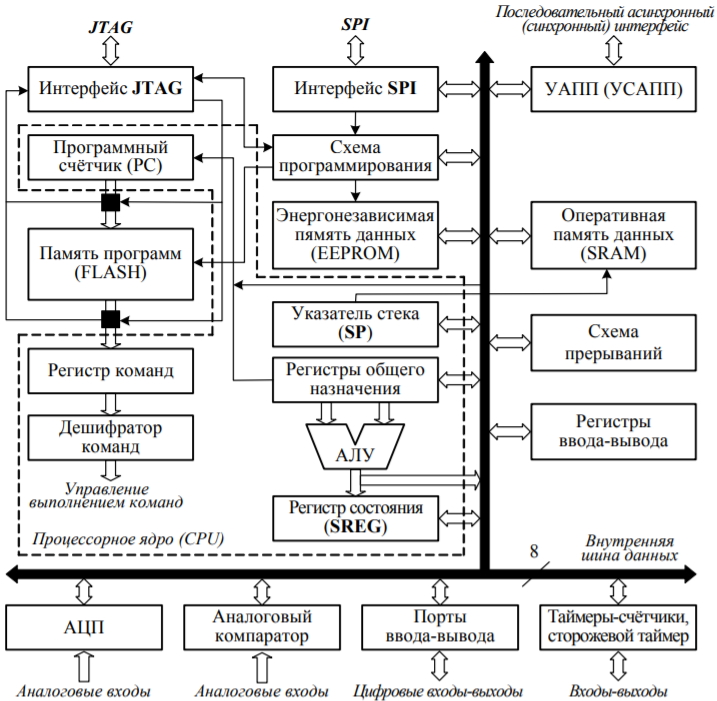
\includegraphics[scale=0.44]{Architecture_AVR.png}
        \caption{Архитектура микроконтроллеров семейства AVR}
        \label{fig:arch_AVR}
    \end{figure}
\end{frame}

\begin{frame}{Архитектура AVR и ARM}
    \begin{figure}
        \centering
        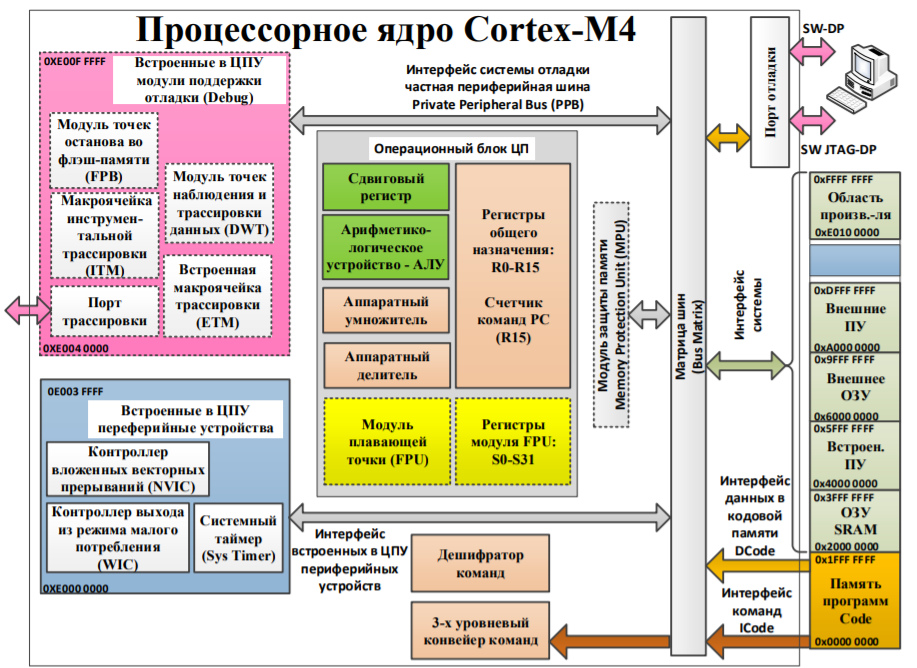
\includegraphics[scale=0.45]{Architecture_ARM.png}
        \caption{Архитектура микроконтроллеров ARM на примере Cortex M4}
        \label{fig:arch_ARM}
    \end{figure}
\end{frame}

\begin{frame}{Идеология RISC в AVR и ARM}
    \setlength{\parindent}{0.5cm}
    Архитектуры AVR и ARM обладают следующими особенностями RISC:
    
    \begin{itemize}
        \item Архитектура загрузки/хранения;
    
        \item Нет поддержки нелинейного доступа к памяти (для некоторых более поздних версий ARM такая возможность была реализована);
    
        \item Равномерный регистровый файл (в AVR микроконтроллерах есть три сдвоенных регистра-указателя);
    
        \item Фиксированная длина команд для упрощения декодирования за счет снижения плотности кода;
    
        \item Одноцикловое исполнение.
    \end{itemize}
\end{frame}

\begin{frame}{Наборы команд AVR и ARM}
    \setlength{\parindent}{0.5cm}
    Система команд микроконтроллеров AVR весьма развита и насчитывает в различных моделях от 90 до 135 различных инструкций.
    
    Все множество команд микроконтроллеров AVR можно разбить на несколько групп:
    
    \begin{itemize}
        \item команды логических операций;
    
        \item команды арифметических операций и команды сдвига;
    
        \item команды операции с битами;
    
        \item команды пересылки данных;
    
        \item команды передачи управления;
    
        \item команды управления системой.
    \end{itemize}
\end{frame}

\begin{frame}{Наборы команд AVR и ARM}
    \setlength{\parindent}{0.5cm}
    В архитектуре ARM, на сегодняшний день, существует несколько наборов команд: ARM, Thumb, Thumb-2, Jazelle, A64.
    
    Микроконтроллеры ARM семейства Cortex M из всех перечисленных наборов команд поддерживают лишь наиболее универсальный Thumb-2.
    
    Набор команд Thumb-2 расширяет набор 16-разрядных команд Thumb дополнительными 32-разрядными, чтобы задать набору команд дополнительную ширину. Цель Thumb-2 --- достичь плотности кода, как у Thumb, и производительности, как у набора команд ARM на 32 битах.
\end{frame}

\begin{frame}{Программная модель AVR-микроконтроллеров}
    \begin{figure}
        \centering
        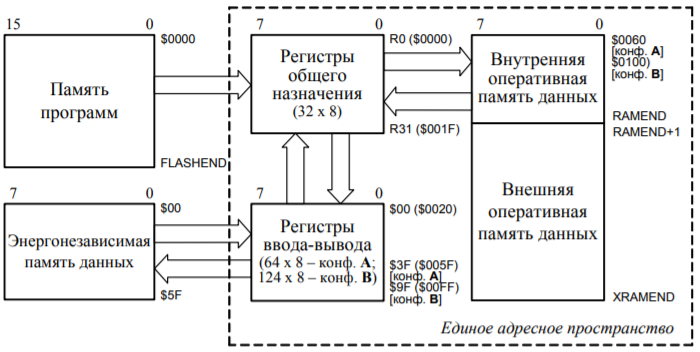
\includegraphics[scale=0.8]{Program_model_AVR.png}
        \caption{Программная модель микроконтроллеров AVR}
        \label{fig:prog_AVR}
    \end{figure}
\end{frame}

\begin{frame}{Программная модель ARM-микроконтроллеров}
    \begin{figure}
        \centering
        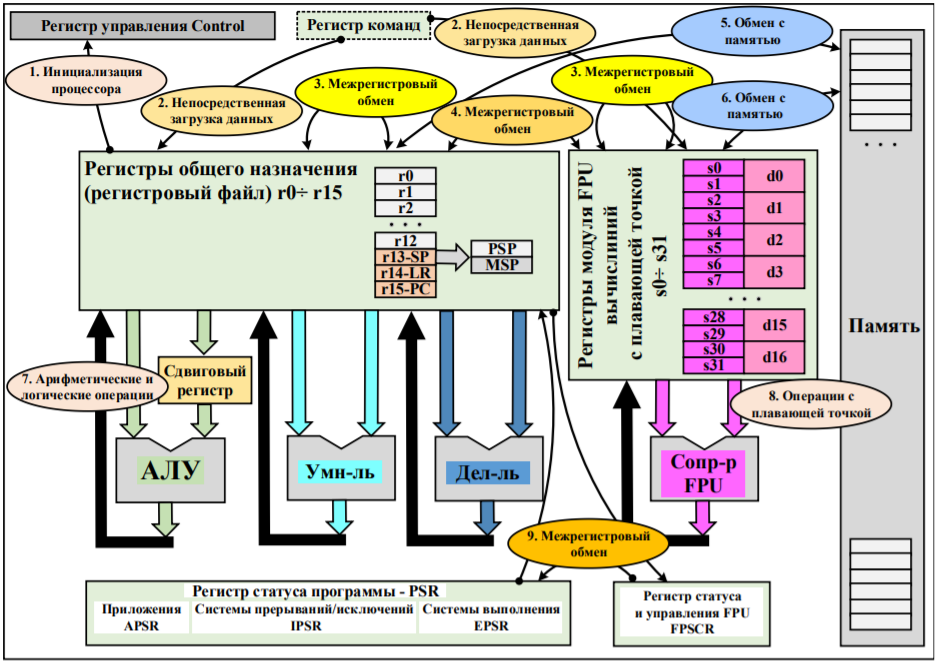
\includegraphics[scale=0.45]{Program_model_ARM.png}
        \caption{Программная модель микроконтроллеров ARM}
        \label{fig:prog_ARM}
    \end{figure}
\end{frame}

\begin{frame}{Периферия микроконтроллеров AVR и ARM}
    \setlength{\parindent}{0.5cm}
    Микроконтроллеры AVR имеют хорошо развитую периферию.
    
    К периферийным устройствам AVR-микроконтроллера относятся многофункциональные, двунаправленные порты ввода-вывода, таймеры, счетчики, сторожевой таймер, аналоговый компаратор, 10-разрядный 8-канальный АЦП (12-разрядный для XMEGA AVR), универсальный асинхронный (синхронно-асинхронный) приемопередатчик --- УАПП (УСАПП), последовательный периферийный интерфейс (SPI), интерфейс JTAG, устройство сброса по понижению питания, широтно-импульсные модуляторы, датчики температуры и др.
\end{frame}

\begin{frame}{Периферия микроконтроллеров AVR и ARM}
    \setlength{\parindent}{0.5cm}
    Перифирия микроконтроллеров с архитектурой ARM также хорошо развита и включает в себя порты ввода-вывода, систему прерываний, АЦП, таймеры общего назначения, сторожевой таймер, расширенный таймер, часы реального времени, последовательный периферийный трехпроводный интерфейс SPI, модуль I2C, модуль УСАПП и др.
\end{frame}

\begin{frame}{Питание  микроконтроллеров AVR и ARM}
    \setlength{\parindent}{0.5cm}
    AVR функционируют при напряжениях питания от 1,8 до 6,0 В.

    AVR могут быть переведены программным путем в один из трех режимов пониженного энергопотребления:
    
    \begin{itemize}
        \item Режим холостого хода
    
        \item Стоповый режим
    
        \item Экономичный режим
    \end{itemize}
    
    В микроконтроллерах существует специальный режим --- сброс при снижении напряжения питания (BOD).
\end{frame}

\begin{frame}{Питание  микроконтроллеров AVR и ARM}
    \setlength{\parindent}{0.5cm}
    Для работы микроконтроллеров ARM их необходимо питать напряжением в диапазоне от 1.2 до 5.5 В.

    ARM микроконтроллер может работать в одном из следующих режимов:
    
    \begin{itemize}
        \item Run
        
        \item Low-Power Run
        
        \item Sleep
        
        \item Low-Power Sleep
        
        \item Stop 0
        
        \item Stop 1
        
        \item Standby With SRAM
        
        \item Standby Without SRAM
        
        \item Shutdown
    \end{itemize}
\end{frame}

\begin{frame}{Arduino. Программная часть}
    \begin{figure}
        \centering
        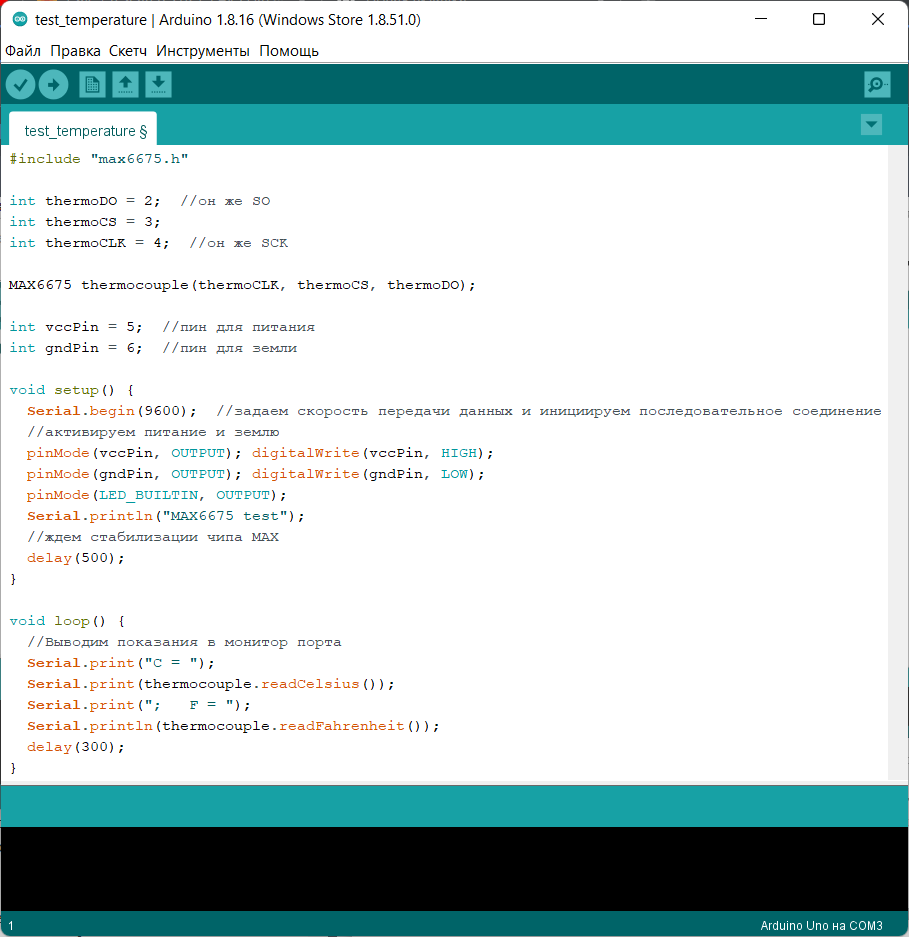
\includegraphics[scale=0.33]{Arduino_IDE.png}
        \caption{Интерфейс Arduino IDE с примером простой программы}
        \label{fig:ide}
    \end{figure}
\end{frame}

\begin{frame}{Arduino. Аппаратная часть}
    \begin{figure}
        \centering
        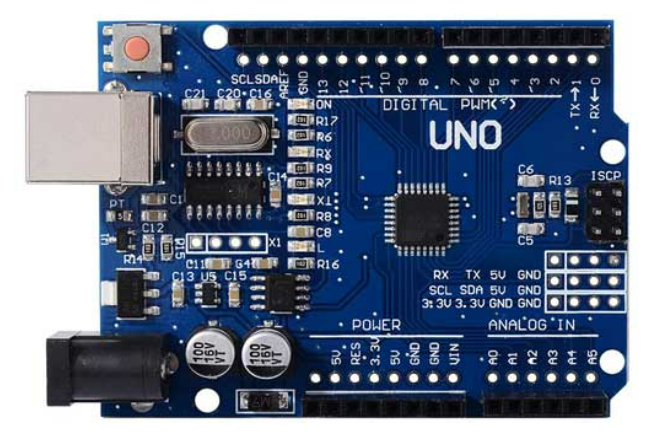
\includegraphics[scale=0.6]{Arduino_Uno.png}
        \caption{Отладочная плата Arduino Uno}
        \label{fig:uno}
    \end{figure}
\end{frame}

\begin{frame}{Заключение}
    \setlength{\parindent}{0.5cm}
    В результате выполнения научно-исследовательской работы были выполнены следующие задачи:

    \begin{enumerate}
        \item Осуществлено знакомство с архитектурой микроконтроллеров AVR и ARM на примере представителя каждого семейства.
        
        \item Осуществлено знакомство с наборами команд для микроконтроллеров семейств AVR и ARM.
        
        \item Изучены некоторые аппаратные и программные средства для разработки под AVR и ARM микроконтроллеры, наиболее подходящие для дальнейшего обучения и разработки на начальном уровне.
    \end{enumerate}
\end{frame}

\end{document}
